\chapter{Design} \label{Chapter:Design}

\section{Specification}

% {\color{red}Specification of works, quantifiable}

\begin{itemize}
	\setlength\itemsep{0em}
	\item Customise a NVIDIA Jetson TK1 embedded board and its Linux operating system for power efficiency.
	\item Interface an OV5647 camera to the target platform through MIPI-CSI interface and V4L2 driver platform.
	\item Configure the camera including different resolution modes through V4L2 interface.
	\item Capture still images and video sequences with the camera through V4L2 interface.
	\item Control the camera frame rate while the camera is actively capturing video stream.
	\item Implement object tracking algorithm on the target platform for video surveillance application.
	\item Optimise the algorithm so that it runs around $30$ FPS on the platform.
	\item Achieve $50\%$ power saving on some typical real world video surveillance dataset through adaptive operation.
	\item Maintaining $80\%$ successful object tracking rate with the adaptive operation.
	\item Build a camera and algorithm power consumption model.
	\item Use the model to estimate power saving achieved through adaptive operation.
\end{itemize}

\section{System block diagram}

\begin{figure}[H]
  \centering
  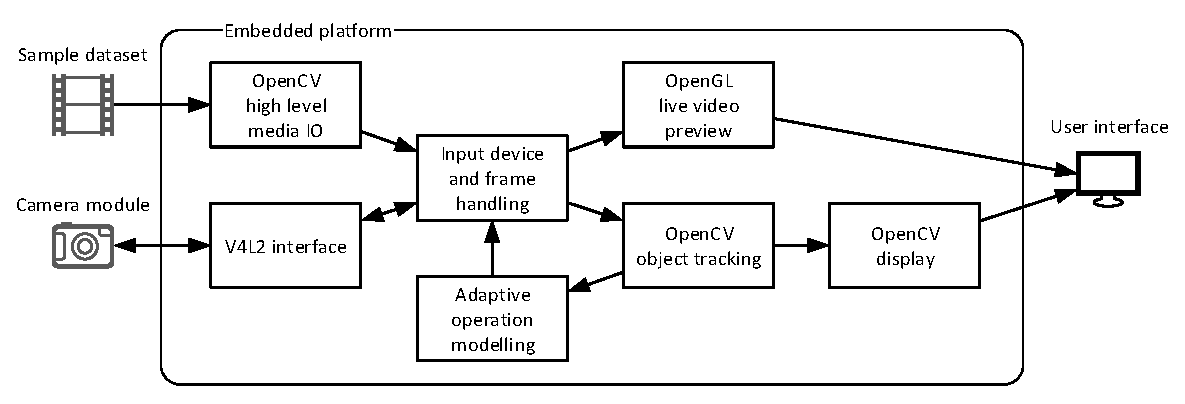
\includegraphics[width=\columnwidth]{block}
  \caption{Purposed system design block diagram.}
  \label{block}
\end{figure}

% {\color{red}BLOCK DIAGRAM}

\section{Hardware}

% {\color{red}Design works, choices of hardware, software, etc.}

\subsection{Hardware platform}

%ARM or x86?

An embedded development board was used in this project, it enables easy power consumption analysis and is more likely the situation where power efficiency will be required rather than a desktop or server environment.

The most broadly used and powerful embedded processor architecture is ARM. It has relatively high performance grade available, extensively hardware and software support including embedded Linux operating system with reasonable power consumption and varies power saving modes, therefore was chosen to be used in this project.

Specifically, the Jetson Tegra K1 embedded development platform \cite{NVIDIA:tk1} featuring a 2.32GHz quad-core ARM CPU and a CUDA enabled Tegra GPU, introduced by NVIDIA, was used in this project. It has a rich set of peripheral interfaces exported enables low-level control and interfacing with a MIPI-CSI high resolution camera module and is powerful enough to develop programs and execute complex computer vision algorithms on board. The heterogeneous architecture with CUDA enabled GPU can also be fully utilised by the GPU module in the specifically optimised OpenCV library, makes it particularly suitable for computer vision tasks.

There are other heterogeneous architecture embedded platforms with ARM CPU cores and ARM GPUs available, but ARM GPUs are currently not supported by OpenCV's GPU module, and the CPUs alone are probably not powerful enough for complex computer vision tasks.

% {\color{red}More}

A general x86 architecture computer running Microsoft Windows operation system with a webcam was also used for algorithm development and remote control of the embedded development board. Since most algorithm developments do not use platform specific features, they can be developed on a general computer then easily migrated to the embedded platform.

\subsection{Camera}

% Specific camera module to be used was not determined yet at the time this progress report was written, but it would be a high resolution camera module from OmniVision \cite{ovt} that can be easily interfaced and directly controlled with the peripheral interfaces on the Jetson TK1 platform. A Linux kernel module driver probably need to be developed in order to control the camera parameters and operations from program running in user space.

The Raspberry Pi camera module was used in this project, it features a 5 mega pixels OV5647 camera sensor manufactured by OmniVision Technologies Inc. It is relatively more expensive than buying the camera sensor only, but the raspberry pi camera module is more broadly available in small quantities and can be easily connected to the board without the need to design a dedicated adapter PCB. It uses the MIPI-CSI interface which the board has native support for, the complete data sheet is also available around the Internet and it features subsampling, frame rate control, auto exposure and white balance functions etc. which are essential to adaptive operation.

The only difficulty is that the camera sensor can only output frames in raw Bayer pattern format \cite{bayer1976color}, as shown by \fref{bayer}. A typical colourful computer image consists of 3 primary colour channels per pixel, which are red, green and blue, i.e. RGB colour space. However, because of physical and manufacture constrains, most of camera sensors including the camera used in this project have only one intensity sensor per pixel with a specific colour filter, arranged in Bayer pattern format, therefore image processing algorithm need to be applied to convert or approximate the raw data to produce full colour images. Some of the camera sensors have a built-in image processor that applies the algorithm automatically, but the Raspberry Pi camera sensor used in this project doesn't have that functionality, therefore the algorithm need to be implemented by the application. But since the format can be efficiently converted using the GPU cores and CUDA, that is not a significant issue.

\begin{figure}[H]
  \centering
  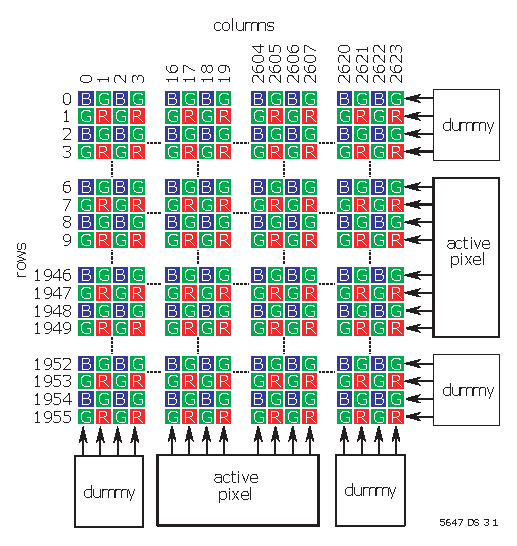
\includegraphics[width=0.6\columnwidth]{bayer}
  \caption{The Bayer pattern pixel arrangement used by the camera module (source from OV5647 datasheet).}
  \label{bayer}
\end{figure}

\section{Software}

\subsection{Operating system}

Ubuntu Linux distribution version 14.04.1 LTS was used on the platform, installed directly from the file system image provided by NVIDIA. Linux is great for this project because it is fully configurable, so that operating system overheads can be reduced to minimum by disabling unused services, even the graphical desktop environment. Also most Linux operations can be done through just command line interface, possibly via a SSH shell access, therefore programming and controlling the platform can be done anywhere with internet connection, which is very convenient.

The open-source GNU/Linux system also provides familiar and widely used tool sets, kernel driver development is well-documented, cross platform computer vision libraries especially OpenCV is also available, and has enormous community support.

\subsection{Computer vision API}

OpenCV \cite{opencv} was used to implement the algorithms, due to its cross platform adaptability, easy to use and has large number of efficient algorithms ready for use and analysis. Furthermore, the OpenCV library for Jetson platform provided by NVIDIA had been further optimised, provides 2x-5x speed up compare to regular OpenCV \cite{NVIDIA:perf}. The OpenCV GPU module based on NVIDIA CUDA was also available, utilises the heterogeneous architecture and provides 5x-20x speed up. These optimisations can reduce computation time dramatically, thus further reduces the power consumption.

\subsection{Testing dataset}

Using a consistent video stream input and a camera power consumption model instead of replaying the same scene in front of the camera is preferred, because reproducing the exactly same video stream from replaying scene is impossible, factors such as camera and object instability, inaccurate synchronisation, hardware and software restrains will also take effect.

The video database from \cite{goyette2012changedetection} was used for testing the algorithms and analysing the performance and accuracy of adaptive operation. The database was rigorous and comprehensive, involves lots of carefully chosen video streams from different real life scenarios, very useful for evaluate object tracking algorithms in different situation.

\section{Algorithms}

\subsection{Object detection algorithm}

The model based object detection algorithms described in previous chapter might be useful for some specific projects, but for a more general object tracking system with previously specified application areas, motion based algorithms which can track any kind of moving objects, was used in this project for evaluating adaptive operation.

There are 2 possible motion based object detection algorithms described previously, background subtraction and optical flow. Since optical flow can only detect moving objects, objects moving in a relatively low speed or stops for a few moments, which are common in a lot of scenarios would be undetectable by optical flow, therefore background subtraction that can handle this kind of situations was used for the object detection phase.

However, there are several distinctive background subtraction algorithms available for use. After some evaluations, the ViBE algorithm was chosen, because it is relatively efficient, with moderate memory usage and has GPU implementation, thus can take the advantage of heterogeneous platform architecture.

\subsection{Object tracking algorithm}

Connected component analysis is used after foreground masks being extracted from each frame. Specifically, the simple find contours function that is also used by the simple blob detector from OpenCV was used. It is very simple, but still sufficient to extract blobs from black and white masks without intensive computation.

Afterwards, the good features to track function is used to determine feature points inside foreground masks, then related to the objects detected respectively. After that, sparse set optical flow will be applied to track the movements of feature points in following frames. By relating the feature points back to objects, the objects can then be tracked.

% {\color{red}HOW???}
